% https://en.wikipedia.org/wiki/Asteroids_(video_game)
% https://en.wikipedia.org/wiki/Golden_age_of_arcade_video_games
% https://www.arcade-museum.com/game_detail.php?game_id=6939
% https://www.ranker.com/list/the-most-popular-golden-age-arcade-games/video-games-lists
% https://stella-emu.github.io/index.html
% https://stella-emu.github.io/docs/index.html
%

% https://github.com/openai/retro
% https://blog.openai.com/gym-retro/
% https://openai.com/
% https://gym.openai.com/

% https://en.wikipedia.org/wiki/TensorFlow
% https://github.com/tensorflow/tensorflow
% https://www.tensorflow.org/
% RUSSEL, Stuart Jonathan and NORVIG, Peter - Artificial Intelligence: a mordern approach

% labels:
% cap:fundamentos
% sec:nn ............ neural network
% sec:dl ............ deep learning
% sec:cnn ........... convolutional neural network
% sec:mdp ........... markov decision process
% sec:rl ............ reinforcement learning
% sec:ql ............ q learning
% sec:aql ........... approximate q learning
% sec:dql ........... deep q learning
% sec:enhance ....... enhancements
% sec:er ............ experience replay
% sec:ft ............ fixed target

%% ---------------------------------------------------------------------------- %
\chapter{Fundamentos}
\label{cap:fundamentos}
%% ---------------------------------------------------------------------------- %

Para se criar e treinar uma inteligência artificial, diversos arcabouçous são necessários.
Por um lado, existe a parte teórica e matemática na qual a inteligência se baseia para aprender. 
Por outro, do lado computacional, existem as bibliotecas que auxiliam no desenvolvimento, efetuando as operações necessárias e, neste trabalho em particular, emulando os ambiente.
Este capítulo tem o intuito de familiarizar o leitor com a teoria e técnicas utilizadas na modelagem e treinamento da inteligência artificial deste trabalho.

% ---------------------------------------------------------------------------- %

\section{Redes neurais}
\label{sec:nn}
%https://www.doc.ic.ac.uk/~nd/surprise_96/journal/vol4/cs11/report.html#What%20is%20a%20Neural%20Network
%https://www.youtube.com/watch?v=aircAruvnKk&list=WL
%https://towardsdatascience.com/the-mostly-complete-chart-of-neural-networks-explained-3fb6f2367464

% https://softwarerecs.stackexchange.com/questions/47841/drawing-neural-networks
% http://alexlenail.me/NN-SVG/index.html

Redes neurais artificiais, mais conhecidas como redes neurais, são uma forma de processamento de informação inspirada no funcionamento do cérebro.
Assim como o órgão no qual foram baseadas, elas possuem uma grande quantidade de elementos de processamento de informação conectados entre si, chamados de neurônios, que trabalham em conjunto para resolver problemas.
Dado que aprendem com exemplos, é considerada uma técnica de aprendizado supervisionado.
Elas são muito utilizadas como aproximadoras de funções desconhecidas, que não são facilmente modeláveis matematicamente.

Com os avanços nos estudos dessa técnica nos últimos anos, diversos tipos diferentes de redes neurais foram desenvolvidos, como redes neurais convolucionais, o tipo utilizado neste trabalho, e redes neurais de memória de curto-longo prazo\footnote{Tradução livre feita pelo autor} (\textit{Long/Short Term Memory}, LSTM), que não será abordada.
Apesar de cada uma ter sua particularidade, redes neurais clássicas possuem duas características principais: a estrutura dividida em \textbf{camadas}, e os \textbf{neurônios} que as compõe.
Existem redes que não são consideradas clássicas pela falta de estrutura em camadas, como Redes de Hopfield (\textit{Hopfield Network}) e Máquinas de Boltzmann (\textit{Boltzmann Machine}), que também não serão discutidas neste trabalho.

%A estrutura de uma rede neural clássica é dividida em \textbf{camadas} que podem ser classificadas de três formas distintas: \textbf{entrada}, \textbf{oculta}, ou \textbf{saída}.
As camadas de uma rede neural são compostas por neurônios e podem ser separadas em três categorias: \textbf{entrada}, \textbf{oculta}, e \textbf{saída}.
Quando um dado é suprido à rede, ele vem no formato de um vetor de forma que os neurônios da camada de \textbf{entrada} recebem seus elementos para serem processados ao longo da rede;
as \textbf{ocultas} realizam o processamento do dado de entrada;
e a de \textbf{saída} devolve um vetor de números que representa o resultado da rede neural para a entrada dada.
%Pode-se dizer que uma rede neural é um aproximador de uma função que mapeia entrada e saída.
Enquanto o formato da entrada e da saída da rede neural determinam seus respectivos números de neurônios, a quantidade de nós nas camadas ocultas são arbitrários, normalmente definidos por meio de tentativa e erro.

\textbf{Neurônios}, ou nós, são funções que recebem, como entrada, a saída de cada neurônio da camada anterior e devolvem um número
%, em geral entre 0 e 1 inclusos,
cujo significado e como são usados variam de acordo com o objetivo da rede.
%A maneira mais comum de se trabalhar com eles é fazendo a combinação linear dos valores dos neurônios de uma camada e, ao passar por uma função de ativação não-linear, determinar quais neurônios da camada seguinte serão ativados.
Cada neurônio das camadas ocultas representa uma característica detectada ao longo do treinamento.
Se essa característica estiver presente na camada de entrada, então o neurônio correspondente será \textbf{ativado}.
A ativação de um ou mais neurônios pode levar à ativação de outros neurônios na camada seguinte e assim sucessivamente.
%Esse é um comportamento inspirado na forma como neurônios do cérebro enviam sinais de um para o outro.
A forma mais comum de se utilizá-los em redes neurais é por meio da \textbf{combinação linear} dos valores dos neurônios de uma camada seguido por uma \textbf{função de ativação}.

Para um neurônio $n$ de uma camada $k$, $k > 0$, que não seja a de entrada, seja $N$, $N > 0$, o número de neurônios da camada anterior $k-1$, $w_{i}$, $i = 1, ..., N$, o peso do $i$-ésimo neurônio da camada $k-1$, e $a_{i}$, $i = 1, ..., N$, o valor de saída do $i$-ésimo neurônio da camada $k-1$.
%, e $b$ o viés \footnote{\textit{bias}, em inglês} da função.
A combinação linear dos neurônios é dada por:

\begin{equation} \label{eq:nn01}
w_{1}a_{1} + w_{2}a_{2} + ... + w_{n}a_{n}
\end{equation}

Antes de ser passada para a função de ativação, é comum, mas não obrigatório adicionar à somatória \ref{eq:nn01} um viés \footnote{\textit{bias}, em inglês} $b$, uma constante que ajuda a melhor aproximar da função desconhecida.
A função de ativação realiza uma transformação não-linear no número que recebe como argumento, a soma de \ref{eq:nn01} com o viés neste caso, para mapear seu resultado em um intervalo e determinar se o neurônio $n$ deve ser ativado ou não.
Tanto a transformação quanto a forma de mapear e o intervalo são determinados pela função utilizada.
%Em seguida, o resultado da somatória \ref{eq:nn01} é passado para a função de ativação, que realiza uma transformação não-linear para mapear essa entrada em um determinado intervalo, como $[0, 1]$ ou $[-1, 1]$, a depender da função utilizada.
%O resultado da função de ativação é utilizado como entrada para um dos nós da camada oculta seguinte.

Esse processo, que consiste em várias multiplicações e adições, precisa ser feito em todos os neurônios das camadas da rede neural, o que pode gerar problemas de ponto flutuante e de tempo de processamento.
Portanto, é conveniente realizar esse processo utilizando matrizes, uma vez que existem diversas bibliotecas com funções que otimizam operações matriciais.
Para um neurônio $n$ de uma camada $k$, $k > 0$, que não seja a de entrada, seja $N$, $N > 0$, o número de neurônios da camada $k-1$, $W$ uma matriz tal que $w_{n, j}$, $j = 1, ..., N$, o peso do $j$-ésimo neurônio da camada $k-1$, $a_{k-1}$ o vetor com os valores de saída dos neurônios da camada $k-1$, e $b$ o viés.
Os valores dos neurônios da camada $k$ podem ser representados como resultado da seguinte operação:

\begin{equation} \label{eq:nn02}
Wa_{k-1} + b
\end{equation}

As funções de ativação mais comuns são a sigmoide (curva logística), ReLU (\textit{Rectified Linear Unit}) e ELU (\textit{Exponential Linear Unit}), sendo a sigmoide a mais antiga e a ELU a mais recente.

O próximo passo é entender como os valores dos neurônios e os respectivos pesos são utilizados para tentar devolver a resposta correta.
%Como mencionado anteriormente, conforme as características se mostram presentes na camada de entrada, os neurônios referentes a esses atributos são ativados até que o neurônio com a resposta dada pela inteligência artificial seja ativado.
Como rede neural é um tipo de aprendizado supervisionado, os exemplos inseridos nela possuem rótulos, saídas esperadas.
%(qual valor que cada neurônio de saída deve ter).
Para que o computador saiba o quão próxima sua resposta estava da correta, é definida uma função de erro, também conhecida como função de custo.
Naturalmente, quanto maior for o erro, mais incorreta foi a previsão.%, e isso permite avaliar o desempenho da rede neural.
%Depois de esse procedimento ser feito com milhares ou até milhões de exemplos, calcula-se a média dos erros obtidos e, com isso, avalia-se o desempenho da inteligência.

Otimizar os pesos de forma a reduzir os erros obtidos com os exemplos parece ser o melhor caminho para melhorar o modelo, mas isso não é necessariamente verdade.
Os exemplos utilizados nessa etapa compõe o \textbf{conjunto de treinamento}.
Se o modelo tiver zero de erro em relação a esse conjunto, ele estará sofrendo de \textit{overfitting}, ou seja, a rede neural se adequa tanto ao conjunto de treinamento que saberá o que fazer apenas nele, estando possivelmente muito diferente da função que se deseja aproximar.
Para determinar o grau de \textit{overfitting}, utiliza-se um \textbf{conjunto de validação}, exemplos diferentes do treinamento que são supridos à rede neural ocasionalmente e que não são utilizados para atualização dos pesos.
Se o erro do conjunto de treinamento diminuir, mas o do conjunto de validação não, então o modelo estará começando a sofrer de \textit{overfitting} e o treinamento deve ser interrompido.
Por fim, utiliza-se um \textbf{conjunto de testes}, exemplos escolhidos pela mesma distribuição de probabilidade que o conjunto de treinamento para fazer uma avaliação do modelo obtido após o treinamento.
Idealmente, um modelo com erro baixo nos três conjuntos não tem problemas de \textit{overfitting} e consegue resolver o problema para o qual foi criado.

De forma resumida, uma rede neural clássica aprende recebendo uma série de números como entrada (exemplo) e devolve uma saída;
calcula-se o quão errada essa saída está em relação ao desejado para aquela determinada entrada (rótulo do exemplo), e ajusta os pesos conforme a necessidade para minimizar o erro;
se a arquitetura da rede tiver sido contruída adequadamente, a IA deverá aprender a resolver o problema para o qual foi feita após exemplos suficientes serem supridos.

% ---------------------------------------------------------------------------- %

\section{Aprendizado profundo}
\label{sec:dl}
%http://www.deeplearningbook.org/
%https://www.cs.toronto.edu/~vmnih/docs/dqn.pdf
%https://machinelearningmastery.com/what-is-deep-learning/
%https://stats.stackexchange.com/questions/182734/what-is-the-difference-between-a-neural-network-and-a-deep-neural-network-and-w

Como explicado anteriormente, redes neurais podem ser divididas em três tipos distintos de camadas: entrada, ocultas, e saída.
Enquanto existe apenas uma camada de entrada e uma de saída, é possível haver mais de uma camada oculta.
Se houver muitas ocultas, a rede neural passa a ser chamada de \textbf{rede neural profunda}.
Atualmente, não existe uma definição exata de quantas camadas são necessárias para uma rede ser classificada como profunda e, mesmo que houvesse, esse número provavelmente mudaria com o passar do tempo.

Uma rede neural profunda que segue o modelo apresentado na seção anterior é chamada de \textit{feedforward} e é o mais típico de \textit{deep learning}.
Ele recebe esse nome pois a informação flui da entrada para a saída sem haver conexões de \textit{feedback} para que a previsão seja feita.
Este tipo de rede neural forma a base para \textbf{redes neurais convolucionais}.%, técnica muito utilizada em visualização e processamento de imagens.
%Como a ideia é treinar uma inteligência artificial que aprende vendo imagens do ambiente, esse foi o tipo escolhido para este trabalho.

\begin{figure}[h!]
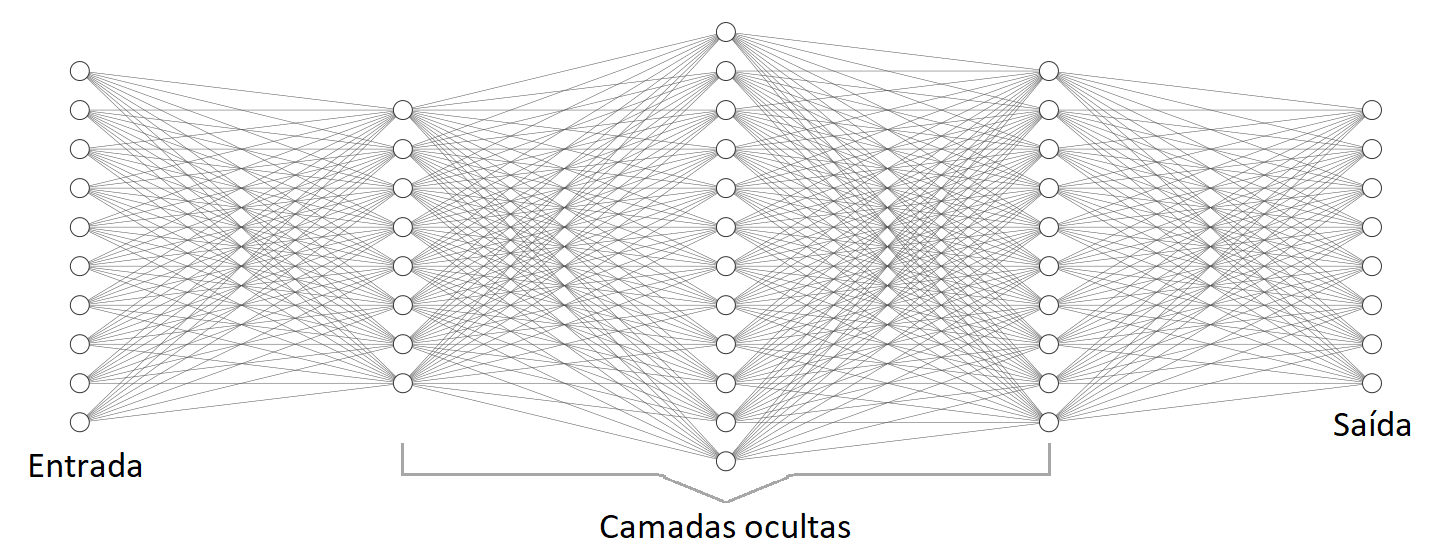
\includegraphics[scale=.3]{nn}
\centering
\caption{Esquema de uma rede neural profunda do tipo \textit{feedforward}. Número de nós e camadas arbitrários para melhor representação. Diagrama feito em \url{http://alexlenail.me/NN-SVG/index.html}}
\end{figure}

% ---------------------------------------------------------------------------- %

\section{Redes neurais convolucionais}
\label{sec:cnn}
%https://medium.com/@ageitgey/machine-learning-is-fun-part-3-deep-learning-and-convolutional-neural-networks-f40359318721

Redes neurais convolucionais (\textit{Convolutional Neural Networks}, CNN) são um tipo de rede neural profunda do tipo \textit{feedforward} especializada em visualização e processamento de imagens.
Sendo uma rede neural clássica, ela possui estrutura dividida em camadas que são formadas por neurônios, com apenas as camadas ocultas funcionando de maneira diferente.
%as de entrada e saída funcionando do mesmo jeito.
%As camadas ocultas, por outro lado, operam de maneira diferente.
Elas podem ser de dois tipos diferentes:
\textbf{convolucionais} ou \textbf{\textit{fully-connected}}.
Enquanto as \textit{fully-connected} funcionam conforme descrito na seção \ref{sec:nn}, com todos seus neurônios conectados a todos da camada anterior, as convolucionais operam de uma forma diferente, tendo duas partes principais:
%Elas possuem duas partes principais:
a \textbf{etapa convolucional}, que dá o nome ao tipo da rede;
e a \textbf{função de ativação}.

A detecção de características de uma CNN é feita na \textbf{etapa convolucional} pelos filtros convolucionais, também chamados de \textit{kernel}, matrizes muito menores que a de entrada, mas com mesmo número de dimensões, que em muitos casos é 3: altura, largura, e canais de cor.
Os filtros convolucionais são os elementos básicos no processamento de imagens, pois são responsáveis por aprender e detectar características nas imagens de entrada.
Eles são deslizados pela matriz de entrada, realizando o produto escalar com a área sobre a qual estão e criando uma nova matriz chamada de \textit{feature map}.
Essa operação é feita para cada filtro e é chamada de convolução.
Após os \textit{feature maps} de cada filtro serem feitos, eles são juntados de forma que a saída da camada tem o formato $N$x$M$x$D$, onde $N$ e $M$ são a altura e largura do \textit{feature map} e $D$ é o número de \textit{kernels}.
A imagem \ref{fig:conv2d} ilustra como convolução ocorre.

\begin{figure}[h!]
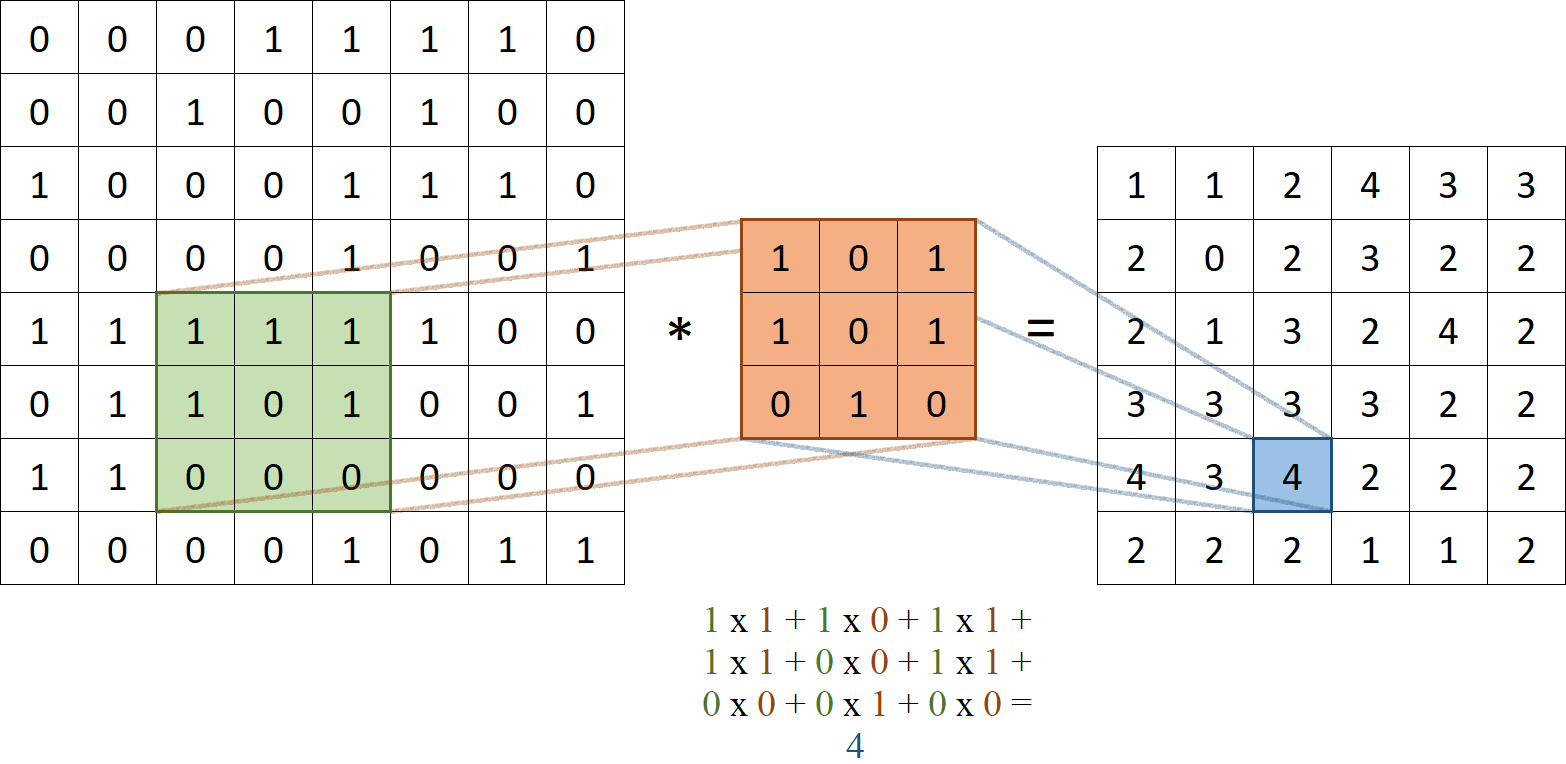
\includegraphics[scale=.275]{conv2d}
\centering
\caption{Exemplo de uma convolução. À esquerda, a matriz de entrada para a camada de convolução; no meio, o filtro; e, à direita, o \textit{feature map} formado. Neste exemplo, a entrada possui apenas um canal de cor, sendo, na prática, uma matriz de duas dimensões.}
\label{fig:conv2d}
\end{figure}

Todos os filtros de uma camada de convolução têm as mesmas dimensões e deslocam-se a mesma quantidade de pixels quando são deslizados para fazer o produto escalar e gerar um ponto do \textit{feature map} correspondente.
O número de filtros por camada, seus tamanhos, e a distância que se movem, também chamada de passo, são hiper parâmetros e, portanto, são definidos previamente pelo desenvolvedor da rede.
Em seguida, aplica-se a \textbf{função de ativação}, em geral a ReLU, em cada elemento de cada \textit{feature map}, resultando na saída da camada convolucional.
É comum, mas não obrigatório utilizar \textit{pooling} depois da função de ativação para reduzir o tamanho dos \textit{feature maps} enquanto preserva as informações importantes, mas essa técnica não foi utilizada neste trabalho.

Por fim, a classificação da entrada é feita pela última camada \textit{fully-connected}, que é a de saída, e avaliada como descrito na seção \hyperref[sec:nn]{Redes Neurais}.
%Camadas \textit{fully-connected} entre as convolucionais e a de saída são consideradas ocultas também.

%Como neste trabalho a IA precisa aprender características do ambiente apenas enxergando imagens dele, utilizar apenas redes neurais profundas sofre de um problema:
%o computador não consegue reconhecer um mesmo objeto em diferentes locais de uma imagem e de diferentes tamanhos como o mesmo.
%Para cada local muito diferente que ele aparecer, como direita e esquerda da tela, a IA teria que re-aprender a identificá-lo.
%
%Como a entrada da rede é uma imagem, uma matriz de pixels, foi utilizada convolução 2D para lidar com o problema descrito acima.
%%Para não precisar fornecer à rede neural imagens inteiras para que ela aprenda que um objeto continua sendo o mesmo não importa onde da tela apareça, foi utilizada convolução, mais precisamente a 2D, já que a entrada é uma imagem, uma matriz de pixels.
%Uma CNN continua sendo um tipo de rede neural profunda e, portanto, mantém o formato de três tipos de camadas (entrada, ocultas, e saída). Porém, para facilitar o entendimento de convolução, esta explicação dividirá a rede em duas partes: \textbf{convolução} e \textbf{previsão}.
%Na etapa de \textbf{convolucão}, a imagem de entrada é dividida em várias imagens menores; elas podem ser adjacentes ou parcialmente sobrepostas, sendo o segundo caso mais comum.
%Cada uma dessas imagens menores é chamada de \textbf{filtro convolucional} ou \textbf{filtro de convolução}.
%É possível dizer que se um filtro convolucional for arrastado para o lado, o local onde ele parar será o próximo filtro convolucional, pois o padrão de pixels deverá ser diferente e, portanto, apresentará uma característica diferente que pode ser detectada.
%Esse arrasto é chamado de passo e a distância que o filtro é arrastado é chamada de tamanho do passo.
%Em seguida, cada uma dessas imagens menores é passada por uma rede neural menor, sendo processada normalmente.
%As saídas dessas redes neurais menores são então passadas como entrada para a próxima etapa.
%Na etapa de \textbf{previsão}, a informação passa por uma ou mais redes neurais maiores que farão a previsão. Para diferenciá-la das redes da etapa de convolução, as desta fase são chamadas de \textit{fully-connected}.
%
%\begin{figure}[h!]
%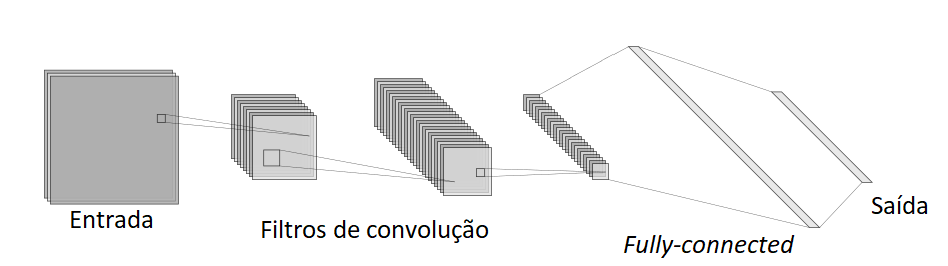
\includegraphics[scale=.4]{cnn}
%\centering
%\caption{Esquema de uma rede neural convolucional. Número de filtros e camadas arbitrários para melhor representação. Diagrama feito em \url{http://alexlenail.me/NN-SVG/LeNet.html}}
%\end{figure}
%
%% ver http://www.deeplearningbook.org/ para resolver a anotação da Nina
É possível haver mais de uma camada de convolução assim como pode haver mais de uma camada \textit{fully-connected} além da de saída, o que pode ser mais vantajoso, uma vez que aumentar a profundidade da rede, em muitos casos, melhora a predição~\cite{Goodfellow-et-al-2016}.
%Quanto mais camadas ocultas houver, mais precisa será a predição.
Entretanto, não só o custo de tempo e de espaço aumentam, como há um limite para o quão melhor será o desempenho da IA.
A partir de um certo ponto, a melhora se torna ínfima em comparação com o tempo desprendido e, portanto, deixa de ser benéfico colocar mais camadas.

%% ---------------------------------------------------------------------------- %

\section{Processo de Decisão de Markov}
\label{sec:mdp}

Antes de falar sobre aprendizado por reforço, é necessário explicar o que é um \textbf{Processo de Decisão de Markov} (\textit{Markov Decision Process} - MDP).
Um MDP padrão possui as seguintes propriedades:
a probabilidade de se chegar em um estado futuro $S'$ dado que a inteligência artificial, também conhecida como agente, se encontra no estado $S$ depende apenas da ação $A$ tomada nesse estado $S$, o que caracteriza a \textbf{propriedade Markoviana};
existe um modelo probabilístico que caracteriza essa transição, dado por $P(S'|S,A)$;
todos os estados do ambiente e todas as ações que o agente pode tomar em cada estado são conhecidas;
e a recompensa é imediatamente recebida após cada ação ser tomada.

\begin{figure}[h!]
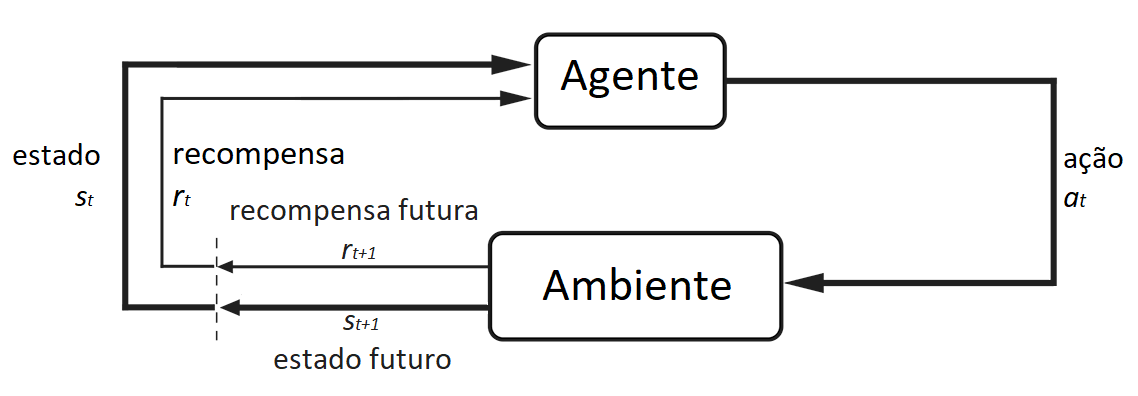
\includegraphics[scale=.45]{reinforcement_learning}
\centering
\caption{Interação agente-ambiente em um processo de decisão de Markov\cite{sutton2018reinforcement}. Adaptação e tradução da imagem original feitas pelo autor.}
\end{figure}

As probabilidades de o agente tomar cada ação em um dado espaço são definidas por uma política $\pi$.
A qualidade de uma política é medida por sua \textbf{utilidade esperada}, e a política ótima é denotada por $\pi^{*}$.
Para calcular $\pi^{*}$, utiliza-se um algoritmo de iteração de valor que computa a utilidade esperada do estado atual:
começando a partir de um estado arbitrário $S$, tal que seu valor esperado é $V(S)$, aplica-se a equação de Bellman até haver convergência de $V(S)$, denotado por $V^{*}(S)$, que é usado para calcular a política ótima $\pi^{*}(s)$.

Seja $i$ a iteração atual, $S$ o estado atual, $S'$ o estado futuro, $A$ a ação tomada no estado atual, $R(S,A,S')$ a recompensa pela transição do estado $S$ para o estado $S'$ por tomar a ação $A$, e $\gamma$ o valor de desconto (valor entre 0 e 1 que determina a importância de recompensas futuras para o agente), temos que:

Equação de Bellman:

\begin{equation} \label{eq:bellman}
V^{(i)}(S) = \max_{A}\sum_{S'}P(S'|S,A)[R(S,A,S') + \gamma V^{(i-1)}(S')]
\end{equation}

\begin{equation} \label{eq:qvalue}
\lim_{i\to\infty} V^{(i)}(S) = V^{*}(S)
\end{equation}

Política gulosa para função valor ótima:

\begin{equation} \label{eq:opt_pol}
\pi^{*}(s) = \argmax_{A}\sum_{S'}P(S'|S,A)[R(S,A,S') + \gamma V^{*}(S')]
\end{equation}

Um processo de decisão de Markov cuja função de probabilidade de transição $P(S'|S,A)$ ou função de recompensa $R(S,A,S')$ é desconhecida se torna um problema de \textbf{aprendizado por reforço}.
%\textbf{Aprendizado por reforço} é um processo de decisão de Markov cuja função de probabilidade de transição $P(S'|S,A)$ ou função de recompensa $R(S,A,S')$ é desconhecida.

%% ---------------------------------------------------------------------------- %

\section{Aprendizado por reforço}
\label{sec:rl}

Aprendizado por reforço, diferente do supervisionado e de redes neurais por consequência, não recebe exemplos rotulados para saber o quão correta ou incorreta sua resposta está para cada entrada.
Ao invés disso, o agente interage com o ambiente e recebe recompensas positivas, negativas ou nulas por suas ações.
Seu objetivo é explorar o espaço de estados a fim de aprender a recompensa esperada para cada ação tomada em cada um deles.
Dessa forma, ele saberá o que fazer em cada situação do ambiente em que se encontra.

As recompensas esperadas de cada ação em cada estado são armazenadas em uma tabela que deve mapear todas as ações para todos os estados.
Isso é possível em domínios simples, como um Jogo da Velha, mas se torna impraticável conforme o espaço de estados aumenta.
No caso do \textit{Pong} e do \textit{Asteroids}, os \textit{frames} do jogo são os estados.
Um pixel que mude de cor já faz ser um estado completamente diferente do ponto de vista do computador.
Em uma tela de 210x160 pixels, com cada pixel armazenando três números que vão de 0 à 255 para determinar sua cor, é evidente não ser possível armazenar na memória um mapeamento das ações para cada um desses estados.
Mesmo que não houvesse esse obstáculo computacional, existem situações em que não é possível determinar qual ação retornará a maior recompensa, como na figura \ref{fig:unknown_best_action}.

\begin{figure}[h!]
%  \begin{minipage}[b]{.45\textwidth}
  \centering
  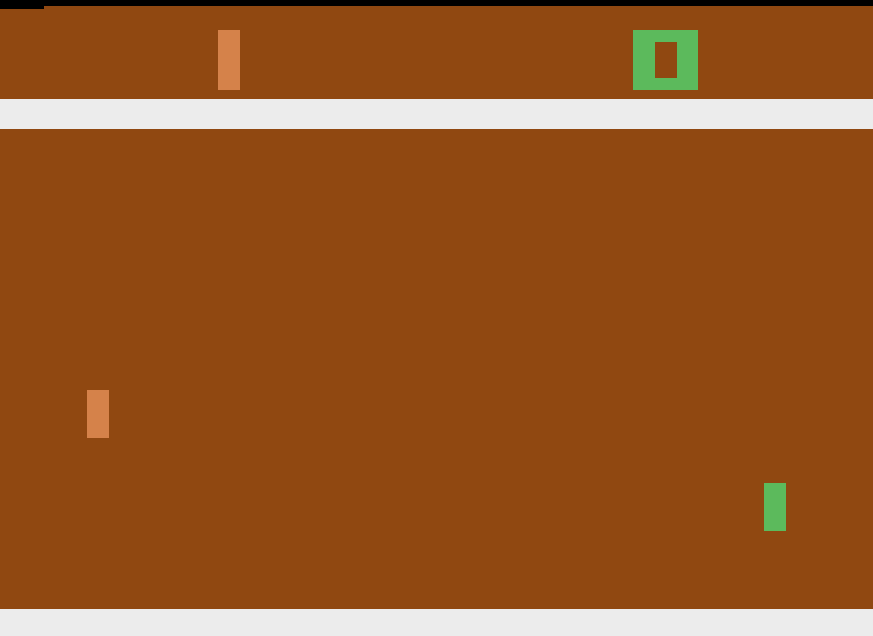
\includegraphics[scale=.275]{pong_unknown_best_action}
%  \end{minipage}
%  \hfill
%  \begin{minipage}[b]{.45\textwidth}
%  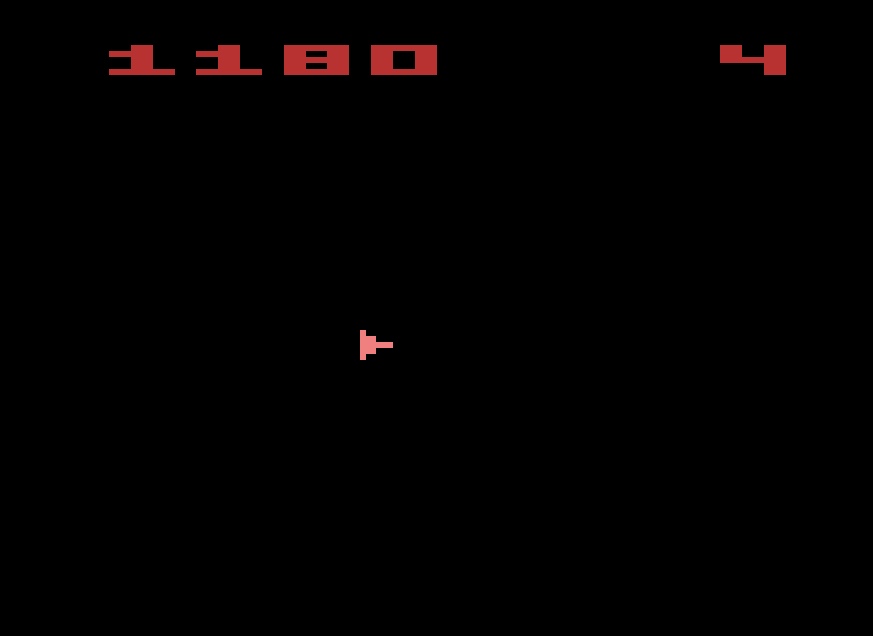
\includegraphics[scale=.275]{asteroids_unknown_best_action}
%  \end{minipage}
%  \centering
  \caption{Quando a bola no \textit{Pong} fica fora da tela, não é possível dizer qual a melhor ação a ser tomada por falta de informação ou porque todas terão o mesmo resultado. No \textit{Pong}, não é possível ver a bola somente quando algum dos jogadores marca um ponto, pois ela saiu da tela pelo lado esquerdo ou direito; quando isso ocorre, todas as ações tomadas têm o mesmo resultado, pois é preciso esperar alguns instantes para uma nova bola aparecer e o jogo continuar.}
  \label{fig:unknown_best_action}
\end{figure}

Como dito no final da seção \hyperref[sec:mdp]{anterior}, aprendizado por reforço é um MDP que não utiliza as probabilidades de transição ou a função de recompensa para aproximar a política ótima.
No contexto deste trabalho, a política ótima será encontrada utilizando uma variante de \textit{\textbf{Q-Learning}}, uma técnica de aprendizado por reforço.

%% ---------------------------------------------------------------------------- %

\section{\textit{Q-Learning}}
\label{sec:ql}

Quando não se conhece as probabilidades de transição ou a função de recompensa, informações necessárias para se obter a função valor pela equação de Bellman, é possível estimar $V(S)$ a partir de observações feitas sobre o ambiente.
Logo, o problema passa a ser como extrair a política do agente de uma função valor estimada.

Seja $Q^{*}(S,A)$ a função Q-valor\footnote{O nome "Q-valor"{} vem do valor da qualidade da ação} que expressa a recompensa esperada de se começar no estado $S$, tomar a ação $A$ e continuar de maneira ótima. $Q^{*}(S,A)$ é uma parte da política gulosa para função valor ótima e é dada por:

\begin{equation} \label{eq:qfunction}
\begin{align*}
Q^{*}(S,A) &= \sum_{S'}P(S'|S,A)[R(S,A,S') + \gamma V^{*}(S')] \\
        &= \sum_{S'}P(S'|S,A)[R(S,A,S') + \gamma \max_{A'}Q^{*}(S',A')]
\end{align*}
\end{equation}

Logo, substituindo \ref{eq:qfunction} em \ref{eq:opt_pol}, temos que a política gulosa ótima para a função Q-valor ótima é dada por:

\begin{equation} \label{eq:q_opt_pol}
\pi^{*}(S) = \argmax_{A}Q^{*}(S,A)
\end{equation}

O próximo passo será entender como atualizar a função Q-valor.
Supondo que o agente se encontra no estado $S$ e toma a ação $A$, que causa uma transição no ambiente para o estado $S'$ e gera uma recompensa $R(S,A,S')$, como computar $Q^{(i+1)}(S,A)$ baseado em $Q^{(i)}(S,A)$ e em $R(S,A,S')$, sendo $i$ o instante atual?
Para responder a essa pergunta, duas restrições precisam ser feitas: $Q^{(i+1)}(S,A)$ deve obedecer, pelo menos de forma aproximada, a equação de Bellman, e não deve ser muito diferente de $Q^{(i)}(S,A)$, dado que são médias de recompensas.
A seguinte equação responde a essa questão.

Seja $\alpha$ a taxa de aprendizado (valor entre 0 e 1 que determina o quão importantes informações novas são em relação ao conhecimento que o agente possui),

\begin{equation} \label{eq:q_update}
\begin{align*}
Q^{(i+1)}(S,A) &= (1-\alpha)Q^{(i)}(S,A) + \alpha[R(S,A,S') + \gamma \max_{A'}Q^{(i)}(S',A')] \\
            &= Q^{(i)}(S,A) + \alpha[R(S,A,S') + \gamma \max_{A'}Q^{(i)}(S',A') - Q^{(i)}(S,A)]
\end{align*}
\end{equation}

A convergência de $Q^{(i)}(S,A)$ em $Q^{*}(S,A)$ é garantida mesmo que o agente aja de forma subótima contanto que o ambiente seja um MDP, a taxa de aprendizado seja manipulada corretamente, e se a exploração não ignorar alguns estados e ações por completo - ou seja, raramente.
Mesmo que as condições sejam satisfeitas, a convergência provavelmente será demasiadamente lenta.
Entretanto, é interessante analisar os problemas levantados pela segunda e pela terceira condição que garantem a convergência e maneiras de solucioná-los.

Se a \textbf{taxa de aprendizado} for muito alta (próxima de 1), a atualização do aprendizado se torna instável.
Por outro lado, se for muito baixa (próxima de 0), a convergência se torna lenta.
Uma solução possível para essa questão é utilizar valores que mudam de acordo com o estado:
mais baixos em estados que já foram visitados muitas vezes, pois o agente já terá uma boa noção da qualidade de cada ação possível, então há pouco que aprender;
e mais altos em estados que foram visitados poucas vezes, pois o agente precisa aprender melhor sobre ele.

Uma vez que a política é gulosa em relação ao Q-valor, o agente sempre tomará a ação que retorna a maior recompensa esperada.
Ou seja, a ação escolhida depende do valor da taxa de desconto $\gamma$: recompensas imediatas serão mais buscadas se for próximo de 0, enquanto recompensas futuras serão mais valorizadas para valores próximos de 1.
Isso é bom somente se todas as recompensas possíveis para aquele estados são conhecidas.
Porém, se houver ações não exploradas, o agente pode perder uma recompensa maior do que as que ele já conhece apenas porque ignorou a ação que leva a ela.
Essa situação caracteriza o dilema \textbf{\textit{Exploration versus Exploitation}}: é melhor tomar a ação que retorna a maior recompensa ou buscar uma melhor?
Da mesma forma que na taxa de aprendizado, uma forma de contornar esse problema é mudar a probabilidade de decidir explorar o ambiente (\textit{explore}) de acordo com a situação.
Conforme o mundo é descoberto, se torna cada vez mais interessante agir de forma gulosa (\textit{exploit}) do que explorar em estados muito visitados, e vice-versa em estados pouco visitados.
Esse comportamento pode ser definido por uma função de exploração.

Seja $P_{ini}$ a probabilidade inicial e $P_{min}$ a probabilidade mínima de o agente decidir explorar (\textit{explore}) o ambiente, $decay$ a taxa de decaimento e $step$ o número de passos dados até o momento.
A probabilidade de o agente explorar (\textit{explore}) o ambiente é dada por:

\begin{equation} \label{eq:exp_exp_prob}
%P_{explore} = P_{min} + (P_{ini} - P_{min})e^{decay * step}
P_{explore} = P_{min} + (P_{ini} - P_{min})e^{-step/decay}
%\begin{cases}
%P_{ini} - decay * step, & \text{se}\ decay * step \leq 0.9 \\
%P_{min}, & \text{caso contrário}
%\end{cases}
\end{equation}

Outro problema enfrentado por \textit{Q-learning} é o de generalização.
A política $\pi^{*}(S)$ determina a melhor ação a se tomar em cada estado.
Logo, utiliza-se uma tabela para armazenar todas essas escolhas.
Porém, como mencionado anteriormente, isso se torna inviável para espaços de estado muito grandes.
Portanto, se não é possível aprender os Q-valores, o melhor que se pode fazer é tentar achar uma aproximação deles.
%Portanto, a solução é generalizar o aprendizado de um estado para o outro: se o agente sabe se comportar em um pequeno conjunto de estados, o ideal é ele saber o que fazer em um estado desconhecido contanto que seja suficientemente parecido com um já aprendido.
%Em outras palavras, o agente aprende propriedades (\textit{features}) dos estados ao invés dos estados propriamente ditos, e toma decisões a partir dessas informações.
%Essa forma de aprender a fazer escolhar é chamada de \textit{\textbf{approximate Q-learning}}.

%% ---------------------------------------------------------------------------- %

\section{\textit{Approximate Q-Learning}}
\label{sec:aql}

\textit{Approximate Q-Learning} é o nome dado a um conjunto de métodos de aprendizado por reforço que busca aproximar o Q-valor das ações.
Uma técnica comum desse conjunto consiste no uso de \textbf{funções lineares} que avaliam características dos estados.

Para lidar com o enorme espaço de estados que alguns ambientes possuem, o agente armazena e aprende apenas algumas propriedades determinadas pelo desenvolvedor, que são funções de valor real, para tomar as decisões.
Tais informações são armazenadas em um vetor e cada elemento desse vetor recebe um peso que determina a respectiva importância para que escolhas sejam feitas. Ou seja, a função Q-valor é representada por uma combinação linear das propriedades e é dada da seguinte forma.

Sejam $f_{i}(S,A)$ e $\omega_{i}$, i = 1, ..., n, a $i$-ésima característica do ambientes detectada pelo agente e seu respectivo peso, ambos representados por números reais.

\begin{equation} \label{eq:q_lin_comb}
Q(S,A) = \omega_{1}f_{1}(S,A) + \omega_{2}f_{2}(S,A) + ... + \omega_{n}f_{n}(S,A)
\end{equation}

Como o $V(S')$ é o valor esperado e $Q(S,A)$ é o valor previsto, a atualização pode ser interpretada como ajustar o Q-valor pela diferença desses dois números.
Além disso, como o \textit{approximate Q-learning} faz uma avaliação das características do estado em que o agente se encontra ($f_{i}(S,A)$) para tomar uma decisão, apenas os pesos ($\omega_{i}$) precisam ser atualizados.

A atualização do $k$-ésimo peso, $\omega_{k}$, $k = 1, ..., n$, ocorre conforme a equação \ref{eq:w_update} abaixo.
%Seja $\omega_{k}^{(i)}$ o peso da $k$-ésima característica no instante $i$; $\alpha$ a taxa de aprendizado; $R(S,A,S')$ a recompensa por se tomar a ação $A$ no estado $S$ para ocorrer transição para o estado $S'$; $\gamma$ a taxa de desconto, 

\begin{equation} \label{eq:w_update}
\omega_{k}^{(i+1)}(S,A) = \omega_{k}^{(i)}(S,A) + \alpha[R(S,A,S') + \gamma V(S') - Q^{(i)}(S,A)]f_{k}(S,A), \hfill k = 1, 2, ..., n
\end{equation}

Duas grandes vantagens de representar o Q-valor como uma combinação linear são evitar \textit{overfitting}, e ser matematicamente conveniente, ter maneiras convenientes de calcular erro e funções que generalizem as decisões.

Percebe-se neste ponto uma semelhança bem grande com a forma como redes neurais profundas funcionam.

%% ---------------------------------------------------------------------------- %

\section{\textit{Deep Q-Learning}}
\label{sec:dql}

Agora que as técnicas de aprendizado profundo e de aprendizado por reforço foram apresentadas, falta falar do tipo de aprendizado obtido quando é feita a junção delas, que é o utilizado neste trabalho: \textit{\textbf{Deep Q-Learning}}.
Por se tratar de um tipo de aprendizado por reforço, mais precisamente \textit{approximate Q-learning}, a inteligência artificial também será referida como agente.

Dado que o agente deve aprender enxergando a tela e tudo que ele vê são matrizes, a primeira etapa consiste em processar essas informações para poder aprender.
Ou seja, o primeiro passo é passar as imagens da tela por uma \textbf{rede neural convolucional}.
Essa etapa funciona conforme descrito na seção sobre \hyperref[sec:cnn]{redes neurais convolucionais}: as imagens são a entrada, ocorre o processamento nas camadas ocultas e, na camada de saída, cada neurônio tem um valor que determinam a ação tomada.
Contudo, calcular o erro é diferente.
Como as imagens passadas não são rotuladas, a IA precisa calcular o erro da saída da rede de outra forma, que será utilizando \textbf{aprendizado por reforço}.
Conforme explicado \hyperref[sec:rl]{anteriormente}, aprendizado por reforço aprende sem o uso de exemplos rotulados, mas precisa que as características que a IA deve aprender estejam bem definidas.
Enquanto tais características são definidas pela rede, o cálculo do erro para a otimização dos pesos é feito pela parte de aprendizado por reforço.

O \textbf{cálculo do erro} é feito por funções que retornam valores altos quando o modelo devolve respostas muito distantes da correta, e próximos de zero caso contrário, como o erro quadrático médio, \textit{cross-entropy} e \textit{Huber loss}~\cite{huber_loss}.
Para minimizar o erro, normalmente utiliza-se o módulo do número retornado pela função de erro, para garantir que será positivo, com alguma variação do \textbf{método do maior declive}, também conhecido como \textbf{método do gradiente}~\cite{cauchy1847} \footnote{\textit{Gradient descent}, em inglês}, como o RMSProp~\cite{rmsprop} e o Adam~\cite{DBLP:journals/corr/KingmaB14}.
Em matemática, gradiente é uma generalização de derivada para múltiplas variáveis e, portanto, aponta para a direção de maior crescimento da função.
O método do gradiente, por outro lado, utiliza o negativo do gradiente para apontar para a direção de maior decrescimento e, por consequência, para um mínimo local.
%O \textbf{cálculo do erro} é feito por uma função que, como toda função, possui um mínimo.
%Esse mínimo é normalmente calculado por alguma variação do \textbf{método do maior declive} ou \textbf{método do gradiente} \footnote{\textit{Gradient descent} em inglês}.
%Em matématica, gradiente é uma generalização de derivada para múltiplas variáveis e, portanto, aponta para a direção de maior crescimento da função sobre a qual foi aplicado no ponto dado.
%Método do gradiente, por sua vez, utiliza o \textbf{negativo} do gradiente para apontar para o mínimo local e, com isso, minimizar o valor da função.

Seja $F(x)$ uma função de múltiplas variáveis, $x_{t}$ um ponto no instante $t$ e $\alpha$ um número real que multiplica o gradiente de $F(x)$.
Em contexto de aprendizado de máquina, $F(x)$ é a função de erro, $x_{t}$ é o vetor de pesos na $t$-ésima iteração e $\alpha$ é a taxa de aprendizado.
A redução do erro é feita atualizando os pesos da seguinte forma:

\begin{equation} \label{eq:error_update}
x_{t+1} = x_{t} - \alpha \nabla F(x_{t})
\end{equation}

Intuitivamente, começa-se em um ponto $x_{0}$ qualquer e utiliza-se esse algoritmo para deslocar-se para um ponto vizinho $x_{1}$ que, se $\alpha$ for pequeno o suficiente, $F(x_{0}) \geq F(x_{1})$.
Se isso for feito iterativamente, tem-se $F(x_{t}) \geq F(x_{t+1})$ a cada passo.
Importante notar que, se o $\alpha$ for muito alto, a redução do erro é rápida, porém instável ou pode sequer acontecer.
Por outro lado, se for muito pequeno, a redução é precisa, mas lenta.
A figura \ref{fig:gradientDescent} ilustra essas situações.

\begin{figure}[h!]
  \begin{minipage}[b]{.45\textwidth}
  \centering
  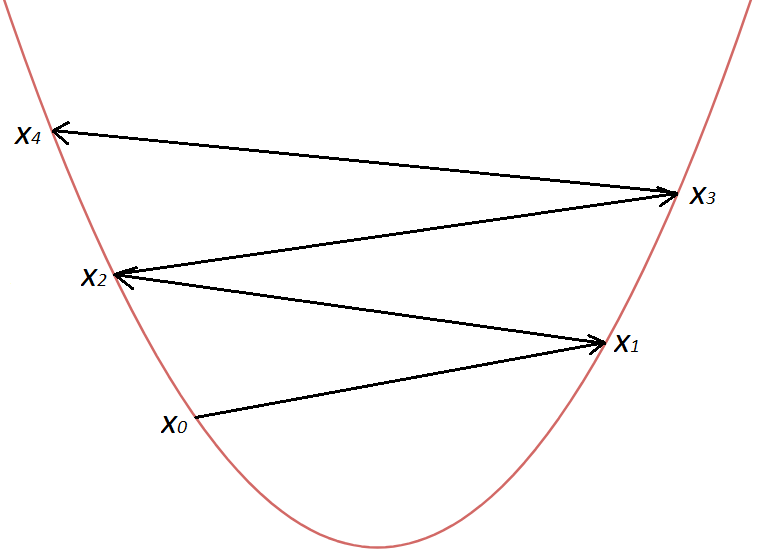
\includegraphics[scale=.15]{gradientDescentHighLR}
  %\caption{A curva representa a função de erro. Se $\alpha$ for muito alto, a diminuição se torna instável ou pode nem ocorrer. Curva desenhada com \url{https://www.desmos.com/calculator}}
  \label{fig:gdhighlr}
  \end{minipage}
  \hfill
  \begin{minipage}[b]{.45\textwidth}
  \centering
  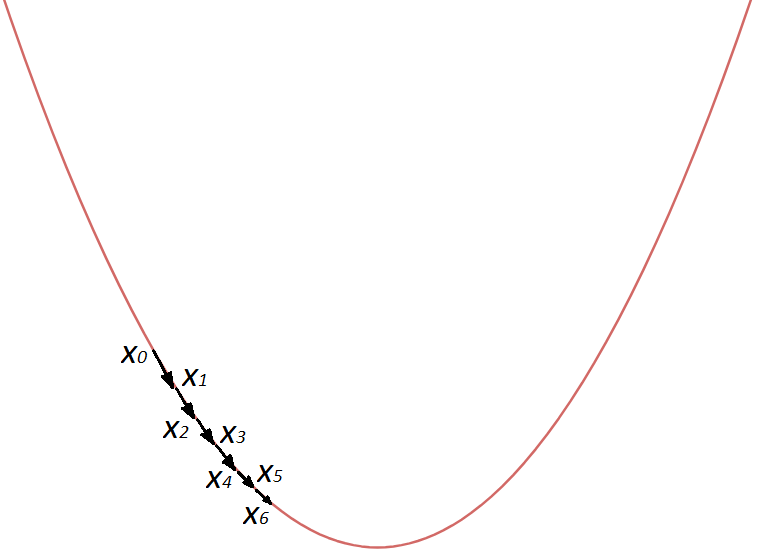
\includegraphics[scale=.15]{gradientDescentLowLR}
  %\caption{A curva representa a função de erro. Se $\alpha$ for muito pequeno, a diminuição se torna precisa, mas lenta. Curva desenhada com \url{https://www.desmos.com/calculator}}
  \label{fig:gdlowlr}
  \end{minipage}
  \caption{Se $\alpha$ for muito alto, a diminuição se torna instável ou pode nem ocorrer (a esquerda); se for muito pequeno, se torna precisa, porém lenta (a direita). Curva representando função de erro desenhada com \url{https://www.desmos.com/calculator}}
  \label{fig:gradientDescent}
\end{figure}

%Existem diversos algoritmos de redução do erro e otimização dos pesos, como o RMSProp, Adam, Adadelta, dentre outros.

%% ---------------------------------------------------------------------------- %

\section{Aprimorando o aprendizado}
\label{sec:enhance}

\textit{Deep Q-Learning} é a base para o aprendizado da inteligência artificial deste trabalho, mas esse processo se torna muito demorado conforme o problema se torna mais complexo.
%Porém, ao longo do tempo, foram descobertas outras técnicas que melhoram a aprendizagem do agente, seja acelerando ou ajudando a evitar decisões ruins.
Nesta seção, serão apresentadas duas técnicas que ajudam a estabilizar e acelerar o aprendizado do programa:
\textit{\textbf{experience replay}}~\cite{Lin1992} e \textbf{alvo fixo}~\cite{humanLevelControlDRL}.

%***********%

\subsection{\textit{Experience replay}}
\label{sec:er}

Estudado inicialmente como um método para acelerar a convergência em aprendizado por reforço, \textit{experience replay} mostrou-se útil para \textit{Deep Q-Learning} por ser uma técnica desse tipo de aprendizagem.
Por conta da forma como \textit{Deep Q-Learning} funciona, se a rede aprendesse com os \textit{frames} conforme o agente os vê, a entrada seria composta por estados sequenciais altamente correlacionados.
Isso significa que ela se atualizaria apenas com as experiências passadas mais recentes, esquecendo as mais antigas e sobrescrevedo os pesos obtidos no passado.
Para contornar esse problema, utiliza-se um \textit{buffer} de memória que armazena uma quantidade pré-determinada de experiências passadas.

Primeiro, o \textit{buffer} de memória é preenchido com $M$ tuplas $t$ de formato $(S, A, R, S', done)$ antes do treinamento, onde $S$ é o estado atual, $A$ é a ação tomada no estado $S$, $S'$ é o estado resultante por se tomar a ação $A$ no estado $S$, $R$ é a recompensa obtida pela transição do estado $S$ para o estado $S'$ como resultado da ação $A$, e $done$ é uma variável que sinaliza se o agente chegou a um estado terminal.
Depois, no treinamento, uma tupla é armazenada na memória a cada passo, enquanto um conjunto de tuplas desse mesmo formato é escolhido aleatoriamente do \textit{buffer} e suprido à CNN para a atualização dos pesos.
%Essas tuplas tem o formato $t = (S, A, R, S', done)$ onde $S$ é o estado atual, $A$ é a ação tomada no estado $S$, $S'$ é o estado resultante por se tomar a ação $A$ no estado $S$, $R$ é a recompensa obtida pela transição do estado $S$ para o estado $S'$ como resultado da ação $A$, e $done$ é uma variável que sinaliza se o agente chegou a um estado terminal.
Dessa forma, o aprendizado ocorre sem o esquecimento de experiências passadas, pois elas são utilizadas para atualização dos pesos a todo momento.
%\textit{Experience replay} também ajuda o agente a tomar ações diferentes ao invés de se prender a algumas que tiveram sucesso no passado próximo e que, possivelmente, não serão tão úteis no futuro.

%***********%

\subsection{Alvo fixo}
\label{sec:ft}
%https://arxiv.org/pdf/1509.02971.pdf

Para o cálculo do erro da ação escolhida pela rede neural, uma comparação definida pela função de erro escolhida é feita entre o Q-valor de saída da rede com um Q-valor alvo calculado a parte.
Sejam $\theta$ os parâmetros da rede neural, $Q_{\theta}$ o Q-valor de saída da rede neural e $\overline{Q}_{\theta}$ o Q-valor alvo.
O Q-valor alvo $\overline{Q}_{\theta}$ e a função de erro são dados, respectivamente, por:

\begin{equation} \label{eq:q_target}
\overline{Q}_{\theta}(S,A) = R(S,A,S') + \gamma max_{A'}Q_{\theta}(S',A')
\end{equation}

%\begin{equation} \label{eq:loss_function}
%L(\theta) = \mathbb{E}[(\overline{Q}_{\theta} - Q_{\theta})^2]
%\end{equation}

Onde $max_{A'}Q_{\theta}(S',A')$ é o maior Q-valor do estado $S'$ calculado pela rede neural com os parâmetros $\theta$.

%Sejam $\theta$ e $\theta_{T}$ os parâmetros da rede principal e da rede alvo respectivamente.
%No início, elas são inicializadas de forma que $\theta = \theta_{T}$.
%A cada passo, apenas $\theta$ é atualizado, enquanto $\theta_{T}$ é atualizado a cada $N$ passos, copiando $\theta$ em $\theta_{T}$.

%Seja $max_{A'}Q(S',A')$ o maior Q-valor do estado S' e $\theta$ os parâmetros da rede neural, o cálculo do erro da ação tomada é feito comparando o Q-valor de saída da rede neural $Q_{\theta}$ com o Q-valor alvo $Q^{T}_{\theta}$, que é dado pela recompensa de se tomar a ação $A$ no estado $S$ e transitar para o estado $S'$ somada ao maior Q-valor de $S'$ multiplicado por uma taxa de desconto $\gamma$.

%\begin{equation} \label{eq:q_target}
%Q^{T}_{\theta}(S,A) = R(S,A,S') + \gamma max_{A'}Q_{\theta}(S',A')
%\end{equation}

%Quando os pesos da rede são otimizados, os Q-valores obtidos por ela aumentam.
%Entretanto, como o $Q_{T}$ também é um Q-valor, a alteração dos parâmetros faz ele aumentar também.
%Consequentemente, se a mesma rede neural for utilizada para calcular o seu Q-valor de saída e o $Q_{T}$ para o cálculo de erro, a comparação será feita entre dois valores que est

Como os mesmos parâmetros da rede são utilizados para calcular o Q-valor de saída e o Q-valor alvo, tanto o $Q_{\theta}$ quanto o $\overline{Q}_{\theta}$ mudam.
Portanto, a otimização dos pesos tenta aproximar a saída da rede de um alvo que está movimento, causanda uma grande oscilação no treinamento, desestabilizando-o.
A solução proposta por \hyperlink{Mni+15}{Mnih et al.(2015)} para amenizar esse problema foi utilizar uma segunda rede neural, inicialmente com os mesmos pesos da rede principal, que é atualizada periodicamente, copiando os parâmetros da principal, ao invés de a cada passo.
Seja $\overline{\theta}$ os parâmetros da rede alvo, o cálculo do erro passa a ser feito utilizando a diferença entre $\overline{Q}_{\overline{\theta}}$ e $Q_{\theta}$.

Com um alvo que se move pouco, a otimização se torna mais estável, melhorando o aprendizado.
%Uma vez que o $Q_{T}(S,A)$ é calculado com os mesmos parâmetros que a rede utilizou para gerar sua saída, quando ela faz os ajustes para aproximar
%Quando os parâmetros da rede são atualizados para que sua saída se aproxime do valor alvo $Q_{T}(S,A)$, por utilizar os mesmos parâmetros para ser calculado, ele também muda

%A inteligência artificial utiliza os Q-valores tanto para decidir quais ações tomar quanto para atualizá-los na tentativa de melhor aproximar o Q-valor real.
%Entretanto, se o mesmo for utilizado para essas duas etapas, o aprendizado se torna instável, pois o agente não conseguirá alcançar o Q-valor alvo já que ele está em constante mudança.
%Para resolver esse problema, utiliza-se uma segunda rede neural alvo para a atualização dos Q-valores e que é atualizada de tempos em tempos, enquanto a primeira, a principal, continua sendo utilizada para escolher as ações.

